~\vskip 10mm
\centerline{\fcolorbox{plum}{white}{\includegraphics[scale=0.59]{9_Page_066.jpg}}}
\vskip 20mm

\titleinline{\textkannada{ಕುರಂತಕನ ಕೈಪಿಡಿ [ಹಠಯೋಗದ ಬಗ್ಗೆ]}}

\centerline{{\large\textkannada{ಪೂಜ್ಯ ಮತ್ತು ಪರಾಕ್ರಮಿ ಗಣಪತಿಗೆ ನಮನಗಳು. ಗುರುಗಳಿಗೆ ನಮನಗಳು}}}
\medskip

\begin{kan}
ಇದು ಸ್ಥಳಾಂತರದ ನೋವಿನಿಂದ ಬಳಲುತ್ತಿರುವವರು, ಇಂದ್ರಿಯ ವಸ್ತುಗಳಿಗೆ ಅತಿಯಾಗಿ ಅಂಟಿಕೊಳ್ಳುವವರು, ಮಹಿಳೆಯರ ಮೇಲೆ ಗೀಳು ಹೊಂದಿರುವವರು, ಜಾತಿಯಿಂದ ಪತಿತರಾದವರು ಮತ್ತು ಅತ್ಯಂತ ಘೋರವಾದ ಕಾರ್ಯಗಳನ್ನು ಮಾಡುವವರ ಹಿತದೃಷ್ಟಿಯಿಂದ ಕಪಾಲಕುರಂತಕ ರಚಿಸಿದ ಹಠ[ಯೋಗ] ಅಭ್ಯಾಸದ ಕುರಿತಾದ ಒಂದು ಕೈಪಿಡಿಯಾಗಿದೆ. ಇದರಲ್ಲಿರುವ ವಿಷಯಗಳು ಮತ್ತು ಅಭ್ಯಾಸದ ತಂತ್ರಗಳನ್ನು [ಇಲ್ಲಿ] ಬರೆಯಲಾಗುವುದು.
\medskip

\heading{\textkannada{[ಯೋಗಿಗಳ] ಗುಡಿಯ ಗುಣಲಕ್ಷಣಗಳು}}


ಅಳತೆಯು ನಾಲ್ಕು ಮುಂಗೈ ಉದ್ದ ಮತ್ತು ಅಗಲವಾಗಿದೆ. ಮುದ್ರೆಗಳ (ಮುದ್ರೆ) ಅಭ್ಯಾಸಕ್ಕಾಗಿ, ಬೂದಿಯಿಂದ [ಡೌಬ್ಡ್] ಮಾಡಿದ ಗುಡಿಸಲನ್ನು [ಬಳಸಬೇಕು]. ಭಂಗಿಗಳ (ಆಸನ) ಅಭ್ಯಾಸಕ್ಕಾಗಿ, ಕೆಂಪು ಮಣ್ಣಿನಿಂದ [ಮಾಡಿದ] ಗುಡಿಸಲನ್ನು. ಎನಿಮಾ (ಬಸ್ತಿ) ನಂತಹ [ಆರು ಶುದ್ಧೀಕರಣ ತಂತ್ರಗಳ] ಅಭ್ಯಾಸಕ್ಕಾಗಿ, ಪ್ಲಾಸ್ಟರ್‌ನಿಂದ [ಡೌಬ್ಡ್] ಮಾಡಿದ ಗುಡಿಸಲನ್ನು. ಮಲಗಲು, ಗುಡಿಸಲಿನಲ್ಲಿ ಹುಲಿಯಂತಹ ಪ್ರಾಣಿಗಳ ಚರ್ಮವಿರಬೇಕು. ವಜ್ರೋಲಿಗೆ, ಹತ್ತಿ ಬಟ್ಟೆ ಮತ್ತು ಅಂತಹುದೇ ಇರಬೇಕು. ಸ್ವರ್ಗಕ್ಕೆ [ಹಗ್ಗದ ಅಗತ್ಯವಿರುವ] ಭಂಗಿಗಳ ಅಭ್ಯಾಸಕ್ಕಾಗಿ, ಅದು ಮೂರು ಬಿಲ್ಲು ಉದ್ದ ಮತ್ತು ಒಂದು ಬಿಲ್ಲಿನ ಉದ್ದ ಅಗಲವನ್ನು [ಅಳತೆ] ಮಾಡಬೇಕು. ಮಲ ವಿಸರ್ಜನೆ ಮತ್ತು ಹೀಗೆ ಮಾಡಲು, ಹತ್ತಿರದಲ್ಲಿ, ಮರೆಮಾಡಿದ ಮತ್ತು ಮುಚ್ಚಿದ ಸ್ಥಳವಿರಬೇಕು. ಸ್ನಾನ ಮಾಡಲು, ಜನರಿಲ್ಲದ ನೀರಿನ ಹೊಳೆ ಇರಬೇಕು.

\heading{\textkannada{ವರ್ತನೆಯ ಸಂಹಿತೆಗಳ ಗುಣಲಕ್ಷಣಗಳು (ಯಮ) ಮತ್ತು ಆಚರಣೆಗಳು (ನಿಯಮ)}}


\textkannada{ಅಹಿಂಸೆ, ಸತ್ಯ, ಕಳ್ಳತನ ಮಾಡದಿರುವುದು, ಅವಲಂಬನೆ ಇಲ್ಲದಿರುವುದು, ನಾಚಿಕೆ, [ಸರಕುಗಳನ್ನು] ಸಂಗ್ರಹಿಸದಿರುವುದು, ನಂಬಿಕೆ, ಬ್ರಹ್ಮಚರ್ಯ, ಮೌನ, ​​ಸ್ಥಿರತೆ, ತಾಳ್ಮೆ ಮತ್ತು ನಿರ್ಭಯತೆ [ಯಮಗಳು]. ಶುದ್ಧತೆ, ಮಂತ್ರಗಳನ್ನು ಪಠಿಸುವುದು, ತಪಸ್ಸು, ಅಗ್ನಿ ಯಜ್ಞ, ವಿಶ್ವಾಸ, ಆತಿಥ್ಯ, ನನ್ನ (ಅಂದರೆ, ದೇವರ) ಪೂಜೆ, ಪವಿತ್ರ ಸ್ಥಳಗಳಿಗೆ ಪ್ರಯಾಣ, ಇತರರಿಗೆ ಸಹಾಯ ಮಾಡಲು ಶ್ರಮಿಸುವುದು, ತೃಪ್ತಿ ಮತ್ತು ಗುರುವಿನ ಸೇವೆ [ನಿಯಮಗಳು].}
\end{kan}

\newpage

~\vskip 1.3cm

\begin{sans}
\titleinline{\color{deepmaroon}{\bfseries\textsanskrit{Kuraṇṭakapaddhatiḥ}}}
\smallskip

\centerline{{\large śrīmahāgaṇapataye namaḥ\!॥ śrīgurubhyo namaḥ\!॥\endnote{The marginal note in the top left corner says, vajrolīyoga\-paddhati\!\textsanskrit{॥} kuraṇṭakapaddhati, voralārtha (?), yogaśāstrārtha.}}}
\smallskip

saṃsārataptānāṃ\endnote{saṃsāra°] P, saṃsārāsāra° M} % 
atyantaviṣayāsaktānāṃ straiṇānāṃ jāti\-bhraṣṭāṇāṃ atisāhasakarmaकर्तॄणां,  tatkṛte iyaṃ kapālakuraṃṭakakṛtahaṭhābhyāsapaddhatiḥ\!।\endnote{°paddhatiḥ] \textit{emend.}, °paddhaty° M} tadgata\-padā\-rthāḥ\endnote{tadgata°] \textit{emend.}, aṃtargata° M} sādhanakarmāṇi\endnote{°karmāṇi] P, °karmāṇī M} ca  likhyante\!।

\textsanskrit{maṭhikālakṣaṇam\!॥}\\ % section heading
caturhastapramāṇamūrdhvaṃ\endnote{ūrdhvaṃ] P, ūrdhva° M} tiryak\!। bhasmamaṭhikā mudrābhyāsārtham\!। āraktamṛttikāmaṭhikā āsanābhyā\-sārtham\!। sudhāmaṭhikā bastyādyabhyāsārtham\endnote{bastyādya°] \textit{conj.}, bastyārthā° M}\!। vyāghrādicarmamaṭhikā śayanārtham\!। tūlavastrādimaṭhikā vajrolyartham\!। tridhanuṣyordhvamekadhanu\-ṣya\-tirya\-ksvargādyāsanārtham\!। samīpaṃ\endnote{samīpaṃ] P, samīpa M} gūḍhaṃ nirvedhaṃ malādityāgārthaṃ sthalam\!। mānuṣarahitajalakulyā snānārtham\!।

\textsanskrit{yamaniyamalakṣaṇam\!॥}\\ % section heading
ahiṃsā satyamasteyamasaṅgo hrīrasañcayaḥ\!।\\
āstikyaṃ brahmacaryaṃ ca maunaṃ\endnote{maunaṃ] P, maunyaṃ M} sthairyaṃ kṣamābhayam\!॥\\
śaucaṃ japastapo homaḥ śraddhātithyaṃ madarcanam\!।\\ %[folio 1v ends at śraddhā]
tīrthāṭanaṃ parārthehā tuṣṭirācāryasevanam\!॥
\end{sans}
\vskip 0.6cm

% [Beginning: English Translation]
\begin{eng}
\centerline{\LARGE\color{deepmaroon}{\textenglish{Kuraṇṭaka's Manual [on Haṭhayoga]}}} % Suggested Heading
\medskip

\centerline{\large Homage to the venerable and mighty Gaṇapati. Homage to the venerable Gurus.} % Separate line (centered?)

This is a manual on the practice of Haṭha[yoga] composed by Kapālakuraṇṭaka for the sake of those afflicted by the pain of transmigration, those excessively attached to sense objects, those obsessed with women, those fallen from caste, and [even] those who perform the most egregious actions. The topics in it and the techniques of the practice shall be written [here].
\bigskip

\heading{\textenglish{Characteristics of the [Yogi's] Hut}}%
The measurement is four forearm lengths high and wide. For the practice of seals (\textit{mudrā}), a hut [daubed] with ash [should be used]. For the practice of postures (\textit{āsana}), a hut [made] of reddish soil. For the practice of the [six cleansing techniques,] such as the enema (\textit{basti}), a hut [daubed] with plaster. For lying down, the hut should have an animal skin, such as that of a tiger. For \textit{vajroli}, it should have a cotton cloth and the like. For the practice of postures [requiring a rope], such as the posture [of Climbing up to] Heaven, it should [measure] three bow lengths high and one bow length wide. For excreting faeces and so on, there should be a place that is nearby, hidden and closed off. For bathing, there should be a stream of water free of people.
\medskip

\heading{\textenglish{Characteristics of the Behavioural Codes (\textit{yama}) and Observances (\textit{niyama})}}
Non-violence, truthfulness, not stealing, non-attachment, shame, not accumulating [goods], belief, celibacy, silence, steadiness, patience and fearlessness [are the  \textit{yama}s]. Purity, reciting mantras, asceticism, [performing] a fire \mbox{sacrifice,} confidence, hospitality, worship of me (i.e., god), travelling to sacred places, striving to help others, satisfaction and serving the teacher [are the \textit{niyama}s].\endnote{\hspace*{.01cm} Both verses were borrowed from the \textit{Bhāgavata\-purāṇa} (11.19.33–34).  In their original context, the compound \textit{madarcana} means `worship of me (i.e., Kṛṣṇa).'}
\end{eng}

\newpage
~\vskip 10mm
\fcolorbox{plum}{white}{\includegraphics[scale=0.68]{9_Page_067.jpg}}
\vskip 20mm

\begin{kan}
\textkannada{ಅಹಿಂಸೆ ಎಂದರೆ ತನ್ನ ದೇಹ, ಮಾತು ಅಥವಾ ಆಲೋಚನೆಯಿಂದ ಇತರರಿಗೆ ನೋವುಂಟು ಮಾಡದಿರುವುದು. ಸತ್ಯವಾದ ಮಾತು ಎಂದರೆ ವಾಸ್ತವಿಕವಾದದ್ದು, ಯಾವುದೇ ಹಾನಿಯನ್ನುಂಟುಮಾಡುವುದಿಲ್ಲ, ಯಾವುದೇ ಉದ್ರೇಕವನ್ನು ಉಂಟುಮಾಡುವುದಿಲ್ಲ ಮತ್ತು ಪ್ರಯೋಜನಕಾರಿಯಾಗಿದೆ. ಕಳ್ಳತನವಲ್ಲದಿರುವುದು ಎಂದರೆ ದೇಹ, ಮನಸ್ಸು ಮತ್ತು ಮಾತಿನಲ್ಲಿ ಇತರರ ಆಸ್ತಿಯ ಮೇಲಿನ ಬಯಕೆಯ ಅನುಪಸ್ಥಿತಿ. [ಯೋಗ] ಅಭ್ಯಾಸವನ್ನು ವಿರೋಧಿಸುವ ಜನರ ಬಗ್ಗೆ ಪ್ರೀತಿ ಇಲ್ಲದಿರುವುದು ಅನಾಸಕ್ತಿ. [ಯೋಗ] ಅಭ್ಯಾಸವನ್ನು ನಾಶಮಾಡುವ ನೀತಿವಂತ ಮತ್ತು ಅನ್ಯಾಯದ [ಕ್ರಿಯೆಗಳಿಗೆ] ನಾಚಿಕೆ ಎಂದರೆ ದುಃಖ. [ಯೋಗ] ಅಭ್ಯಾಸಕ್ಕೆ ಅಗತ್ಯವಿರುವ ವಸ್ತುಗಳಿಗಿಂತ ಭಿನ್ನವಾದ ವಸ್ತುಗಳನ್ನು ಸಂಗ್ರಹಿಸದಿರುವುದು ಎಂದರೆ. ನಂಬಿಕೆ ಎಂದರೆ ಮತ್ಸ್ಯೇಂದ್ರ, ಗೋರಕ್ಷ, ಕಾಕಿ, ಕಾಪಾಲಿಕ ಮತ್ತು ಇತರ [ಪರಿಪೂರ್ಣ ಯೋಗಿಗಳ] ಗ್ರಂಥಗಳಲ್ಲಿ ವಿಶ್ವಾಸ. ಬ್ರಹ್ಮಚರ್ಯ ಎಂದರೆ ಶಿಶ್ನದ ತೆರೆಯುವಿಕೆಯ ಮೂಲಕ ಒಂದು ಹನಿ ವೀರ್ಯ ಬೀಳದಿರುವುದು ಮತ್ತು ಸ್ತ್ರೀ ಉತ್ಪಾದಕ ದ್ರವ ಮತ್ತು [ಇತರ ವಸ್ತುಗಳು] [ಮೂತ್ರನಾಳದ ಮೂಲಕ] ಹೊರಹೋಗುವುದು. ಮೌನವು ಲೌಕಿಕ ವಿಷಯಗಳ ಬಗ್ಗೆ ಮಾತನಾಡುವುದನ್ನು ತಪ್ಪಿಸುವುದು. ಸ್ಥಿರತೆ ಎಂದರೆ ಹೆಂಡತಿ, ಮಗ ಮತ್ತು [ಕುಟುಂಬ]ವನ್ನು ನೋಡಿಕೊಳ್ಳುವ ಬಗ್ಗೆ ಚಿಂತಿಸದೆ ಮನಸ್ಸಿನ ನಿಶ್ಚಲತೆ. ಕಳ್ಳರು, ರಾಜರು ಮತ್ತು ಕೆಟ್ಟ ಜನರಿಂದ ದೈಹಿಕ ಮತ್ತು ಮಾನಸಿಕ ನೋವು ಉಂಟಾದಾಗ ಮತ್ತು ಅವರನ್ನು ಶಿಕ್ಷಿಸುವ ಅಧಿಕಾರವಿದ್ದಾಗ ತಾಳ್ಮೆ ಅಗತ್ಯ. ದೇಹವು ಅಹಂಕಾರದ ಸ್ಥಳವಾಗಿದೆ ಮತ್ತು ಒಬ್ಬರ ಪುತ್ರರು ಮತ್ತು ಮಾಲೀಕತ್ವದ ಪ್ರಜ್ಞೆಗೆ ಸ್ಥಾನವಾಗಿರುವ ಮನೆಗಳು ಇತ್ಯಾದಿಗಳು ಅಶಾಶ್ವತವಾಗಿವೆ ಮತ್ತು ಸತ್ಯ, ಪ್ರಜ್ಞೆ ಮತ್ತು ಆನಂದವಾಗಿರುವ ಸ್ವಯಂ ಶಾಶ್ವತವಾಗಿದೆ ಎಂದು ತಿಳಿದುಕೊಳ್ಳುವುದರಿಂದ ಭಯಪಡದಿರುವುದು ನಿರ್ಭಯತೆ.}

% New paragraph. Start of the niyamas
\textkannada{ಶುದ್ಧತೆ ಎಂದರೆ ದೇಹವನ್ನು ಶುದ್ಧೀಕರಿಸುವುದು [ಶುದ್ಧೀಕರಣ ತಂತ್ರಗಳು], ಉದಾಹರಣೆಗೆ ಎನಿಮಾಗಳು, ಬಟ್ಟೆಯ ಪಟ್ಟಿಯನ್ನು ನುಂಗುವುದು ಮತ್ತು ವಾಂತಿ; ದೇವರ ನಾಮಗಳನ್ನು ಹಾಡುವ ಮೂಲಕ ಮಾತಿನ ಶುದ್ಧೀಕರಣ; ಮತ್ತು ದೇವರನ್ನು ಧ್ಯಾನಿಸುವ ಮೂಲಕ ಮನಸ್ಸಿನ ಶುದ್ಧೀಕರಣ.}
% [End: Kannada Translation]
\end{kan}

\newpage

~\vskip 1cm

\begin{sans}
kāyavāṅmanobhiḥ pareṣāṃ duḥkhadānābhāvaḥ \textbf{ahiṃsā}\!। yathārthaṃ\endnote{yathārthaṃ] P, yāthārthyaṃ M}
ghātāprāpakaṃ anudvegakaraṃ hitaṃ bhāṣaṇaṃ \textbf{satyam}\!। śarīramanovāgbhiḥ paravastvabhilāṣābhāvaḥ \textbf{asteyam}\!। abhyāsapratiyogijanānāmasnehaḥ  \textbf{asaṅgaḥ}\!। abhyāsanāśakeṣu dharmādharmeṣu lajjā \textbf{hrīḥ}\!। abhyāsopayogivastvanyavastusaṅgrāhābhāvaḥ\endnote{°grāhā°] P, ++ (damaged) M} \textbf{asañcayaḥ}\!। matsyendragorakṣakākikāpālikādīnāṃ śāstreṣu viśvāsaḥ \textbf{āstikyam}\!। upasthadvārā vīryabindorapatanaṃ raja[-]ādyākarṣaṇaṃ ca \textbf{brahmacaryam}\!। grāmyaviṣayakathāvivarjanaṃ \textbf{maunam}\!। dāraputrādipālanācintayā\endnote{dāra°] \textit{emend.}, dārā° M. °ācintayā] \textit{conj.}: °acintayā M} manaso 'cāñcalyaṃ \textbf{sthairyam}\!। śārīramānasacorarājaduṣṭajanaduḥkhe teṣāṃ daṇḍakaraṇasāmarthye sati tatsahanaṃ \textbf{kṣamā}\!। ahaṃkārāspadaśarīrādi mamatvādisthānaputragṛhādi anityam,  ātmā nityaḥ saccidānandaśceti jñānena nirbhayatvam \textbf{a\-bhayam}\!।

bastidhautigajakaraṇādinā\endnote{°karaṇādinā] P, karṇādinā M} śarīraśuddhiḥ, bhagavannāmasaṃkīrtanena vākśuddhiḥ, bhagavaddhyānena\endnote{bhagavad°] P, bhagava° M} mānasaśuddhiḥ \textbf{śaucam}\!।
\end{sans}
\vskip 1cm

\begin{eng}
\textbf{Non-violence} is not causing suffering to others with one's body, speech or thought. \textbf{Truthfulness} is speech that is factual, leads to no harm, causes no agitation and is beneficial. \textbf{Not stealing} is the absence of desire for the possessions of others in body, mind and speech. \textbf{Non-attachment} is the absence of affection towards people who oppose the practice [of yoga]. \textbf{Shame} is compunction for righteous and unrighteous [actions] that destroy one’s practice [of yoga]. \textbf{Not accumulating} is not collecting goods that are different to those needed for the practice [of yoga]. \textbf{Belief} is confidence in the scriptures of Matsyendra, Gorakṣa, Kāki, Kāpālika and other [perfected yogis].\endnote{It is not clear who Kāki and Kāpālika might be, or whether kākikāpālika was the intended name. In fact, it seems somewhat likely that the compound \textit{°kākikāpālika°} is a corruption of \textit{°khaṇḍakāpālika°}, the name of a \textit{siddha} mentioned in some manuscripts of the \textit{Haṭhapradīpikā} (1.8).} \textbf{Celibacy} is when not [even] a drop of semen falls through the opening of the penis, and female generative fluid and [other substances] are drawn up [through the urethra]. \textbf{Silence} is avoiding talk about worldly matters. \textbf{Steadiness} is the stillness of mind [brought about] by not worrying about caring for a wife, son and [family]. \textbf{Patience} is that forbearance [required] when physical and mental suffering is caused by thieves, kings and bad people and when one has the power to punish them. \textbf{Fearlessness} is not being afraid as a result of knowing that the body as the locus of ego and one's sons and houses as the seat for the sense of ownership, etc., are impermanent, and that the self, which is truth, consciousness and bliss, is permanent.

\textbf{Purity} is purification of the body by [cleansing techniques], such as enemas, swallowing a strip of cloth, and emesis; purification of speech by singing the names of god; and purification of mind by meditating on god. 
\end{eng}

\newpage

~\vskip 10mm
\fcolorbox{plum}{white}{\includegraphics[scale=0.62]{9_Page_068.jpg}}
\vskip 20mm

% [Beginning: Kannada Translation]
\begin{kan}
ಮಂತ್ರ ಪಠಣ ಎಂದರೆ ಪೂಜಿಸಬೇಕಾದ ದೇವತೆಯ ಮಂತ್ರದ ನಿಯಮಿತ ಪುನರಾವರ್ತನೆ. ತಪಸ್ವಿ ಎಂದರೆ ಒಬ್ಬರ ಧಾರ್ಮಿಕ ಕರ್ತವ್ಯವನ್ನು (ಸ್ವಧರ್ಮ) ನಿರ್ವಹಿಸುವುದು. ಗೃಹಸ್ಥ, ಬ್ರಹ್ಮಚಾರಿ ವಿದ್ಯಾರ್ಥಿ ಮತ್ತು ವನ ಸನ್ಯಾಸಿಗಳಿಗೆ, ಅಗ್ನಿಯಜ್ಞವು ದೈನಂದಿನ ಅಗ್ನಿಯಜ್ಞವಾಗಿದೆ; ತಪಸ್ವಿಗಳಿಗೆ, ಬ್ರಾಹ್ಮಣರಿಗೆ ಹೆಸರಿಗೆ ಮಾತ್ರ, ಮಹಿಳೆಯರು ಮತ್ತು ಅಂತಹವರಿಗೆ, ಇದು ವೈಷ್ಣವ ತಂತ್ರಗಳಲ್ಲಿ ದೇವರ ಆರಾಧನೆಯೊಳಗೆ ಸಹಾಯಕವಾಗಿರುವ ಅಗ್ನಿಯಜ್ಞವಾಗಿದೆ. [ಧರ್ಮಗ್ರಂಥಗಳಲ್ಲಿ, ಉದಾಹರಣೆಗೆ] ಬೋಧಿಸಿದ ನಿಯಮಗಳನ್ನು ಅನುಸರಿಸಲು ಆತ್ಮವಿಶ್ವಾಸವು ಉತ್ಸುಕತೆಯಾಗಿದೆ. ಆತಿಥ್ಯ ಎಂದರೆ ಹಠಯೋಗದಂತಹ ಒಬ್ಬರ ಸ್ವಂತ ಮಾರ್ಗದ ವಿಧಾನಗಳನ್ನು ಅಭ್ಯಾಸ ಮಾಡಿದವರ ಕಡೆಗೆ ದಯೆ. [ನನ್ನನ್ನು ಆರಾಧಿಸುವುದು] ಎಂದರೆ ದೇವರನ್ನು ಆರಾಧಿಸುವುದು, [ಅಂದರೆ,] ಎಲ್ಲಾ ಜೀವಿಗಳ ಬಗ್ಗೆ ಕರುಣೆ, ಯಾವುದರಲ್ಲೂ ಸಂಪೂರ್ಣ ತೃಪ್ತಿ ಮತ್ತು ಎಲ್ಲದರಲ್ಲೂ ಆತ್ಮವನ್ನು ನೋಡುವುದು. [ಯೋಗದ] ಅಭ್ಯಾಸವನ್ನು ಪರಿಪೂರ್ಣಗೊಳಿಸಿದವರನ್ನು ನೋಡಲು ಪವಿತ್ರ ಸ್ಥಳಗಳಿಗೆ ಪ್ರಯಾಣ ಮಾಡುವುದು. ಇತರರಿಗೆ ಸಹಾಯ ಮಾಡಲು ಶ್ರಮಿಸುವುದು ವಿದ್ಯಾರ್ಥಿಗಳು ಅಭ್ಯಾಸದಲ್ಲಿ ಯಶಸ್ವಿಯಾಗಲು [ಸಹಾಯ] ಮಾಡುವ ಗುರಿಯನ್ನು ಹೊಂದಿರುವ ಪ್ರಯತ್ನವಾಗಿದೆ. ತೃಪ್ತಿ ಎಂದರೆ ಆಕಸ್ಮಿಕವಾಗಿ ಸಿಕ್ಕಿದ್ದರಲ್ಲಿ ಸಂತೃಪ್ತಿ. ಗುರುವಿನ ಸೇವೆ ಎಂದರೆ ಶಾಸ್ತ್ರಗಳಲ್ಲಿ ಮತ್ತು ಯೋಗಾನುಭವದಲ್ಲಿ ಆಳವಾಗಿ ಪಾರಂಗತರಾದ ಗುರುವಿನ ಅನುಗ್ರಹವನ್ನು ಪಡೆಯುವುದು.
\bigskip

\heading{\textkannada{[ಭಂಗಿಗಳು (\textit{ಆಸನ})]}} % heading/new section
ಮುಂದೆ, ಆರು ಶುದ್ಧೀಕರಣ ತಂತ್ರಗಳನ್ನು [ಅಭ್ಯಾಸ ಮಾಡುವ] ಸಾಮರ್ಥ್ಯವನ್ನು ಪಡೆಯುವ ಭಂಗಿಗಳನ್ನು ವಿವರಿಸಲಾಗಿದೆ.
\end{kan}

\newpage

~\vskip 1cm

\begin{sans}
upāsyadevatāmantrasya nityāvartanaṃ \textbf{japaḥ}\!। svadharmācaraṇaṃ \textbf{tapaḥ}\!। nityahomaḥ gṛhasthāśramiṇāṃ brahmacāriṇāṃ vānaprasthānāṃ ca\endnote{ca] P, \textit{omitted.} M}, yatīnāṃ brahmabandhustryādīnāṃ\endnote{brahma°] P, braṃha° M} vaiṣṇavatantrādibhagavatpūjāṅgahomaḥ \textbf{homaḥ}\!। śāstraśrutavidhikaraṇautsukyaṃ \textbf{śraddhā}\!। svamārgahaṭhādiyuktyabhyastānāṃ satkāraḥ \textbf{ātithyam}\!। sarvabhūteṣu dayā, yena kena santuṣṭiḥ, sarvatrātmānudarśanaṃ bhagavatpūjā\!।  abhyāsasiddhānāṃ darśanārthaṃ deśe deśe  paryaṭanaṃ \textbf{tīrthāṭanam}\!। śiṣyābhyāsasiddhyarthaṃ\endnote{°siddhy°] P, °sidhy° M} yatnaḥ \textbf{parārthehā}\!। yadṛcchayā prāptena santoṣaḥ \textbf{tuṣṭiḥ}\!। śāstraniṣṇātānubhavaniṣṇātaguroḥ anugrahasaṃpādanam \textbf{ācāryasevanam}\!।
\medskip

{\textsanskrit{[āsanāni\!॥]}}\\ % heading 
atha ṣaṭkarmayogyatāpratipādanāya āsanāni likhyante\!।
\end{sans}
\vskip 1cm

% [End: folio 2v, tiff no. 68]
% [Beginning: English Translation]
\begin{eng}
\textbf{Mantra recitation} is the regular repetition of the mantra of the deity to be worshipped. \textbf{Asceticism} is carrying out one's religious duty (\textit{svadharma}). For the householder, celibate student and forest hermit, a \textbf{fire sacrifice} is the daily fire sacrifice;  for ascetics, Brahmins only in name, women and the like, it is the fire sacrifice that is an ancillary within the worship of god in [scriptures, such as] Vaiṣṇava Tantras. \textbf{Confidence} is eagerness for following the rules taught in scripture. \textbf{Hospitality} is kindness towards those who have practised the methods of one’s own path, such as Haṭhayoga. [\textbf{Worship of me}] is worshipping god, [that is,] compassion for all beings, complete contentment with anything, and seeing the self in all things. \textbf{Travelling to sacred sites} is going to various places for the sake of seeing those who have perfected the practice [of yoga].  \textbf{Striving to help others} is effort directed at [helping] students succeed at the practice.  \textbf{Satisfaction} is contentment with what has been obtained by chance. \textbf{Serving the teacher} is procuring the favour of a teacher who is deeply versed in scripture and the experience [of yoga].
\bigskip

\heading{\textenglish{[Postures (\textit{āsana})]}} % heading/new section
Next, the postures for attaining the capacity for [practising] the six cleansing techniques are described.
\end{eng}



%\newpage
%\thispagestyle{empty}
%\begin{tikzpicture}[overlay, remember picture]
  %\node[inner sep=0pt, minimum width=\paperwidth, minimum height=\paperheight] at (current page.center) {
    %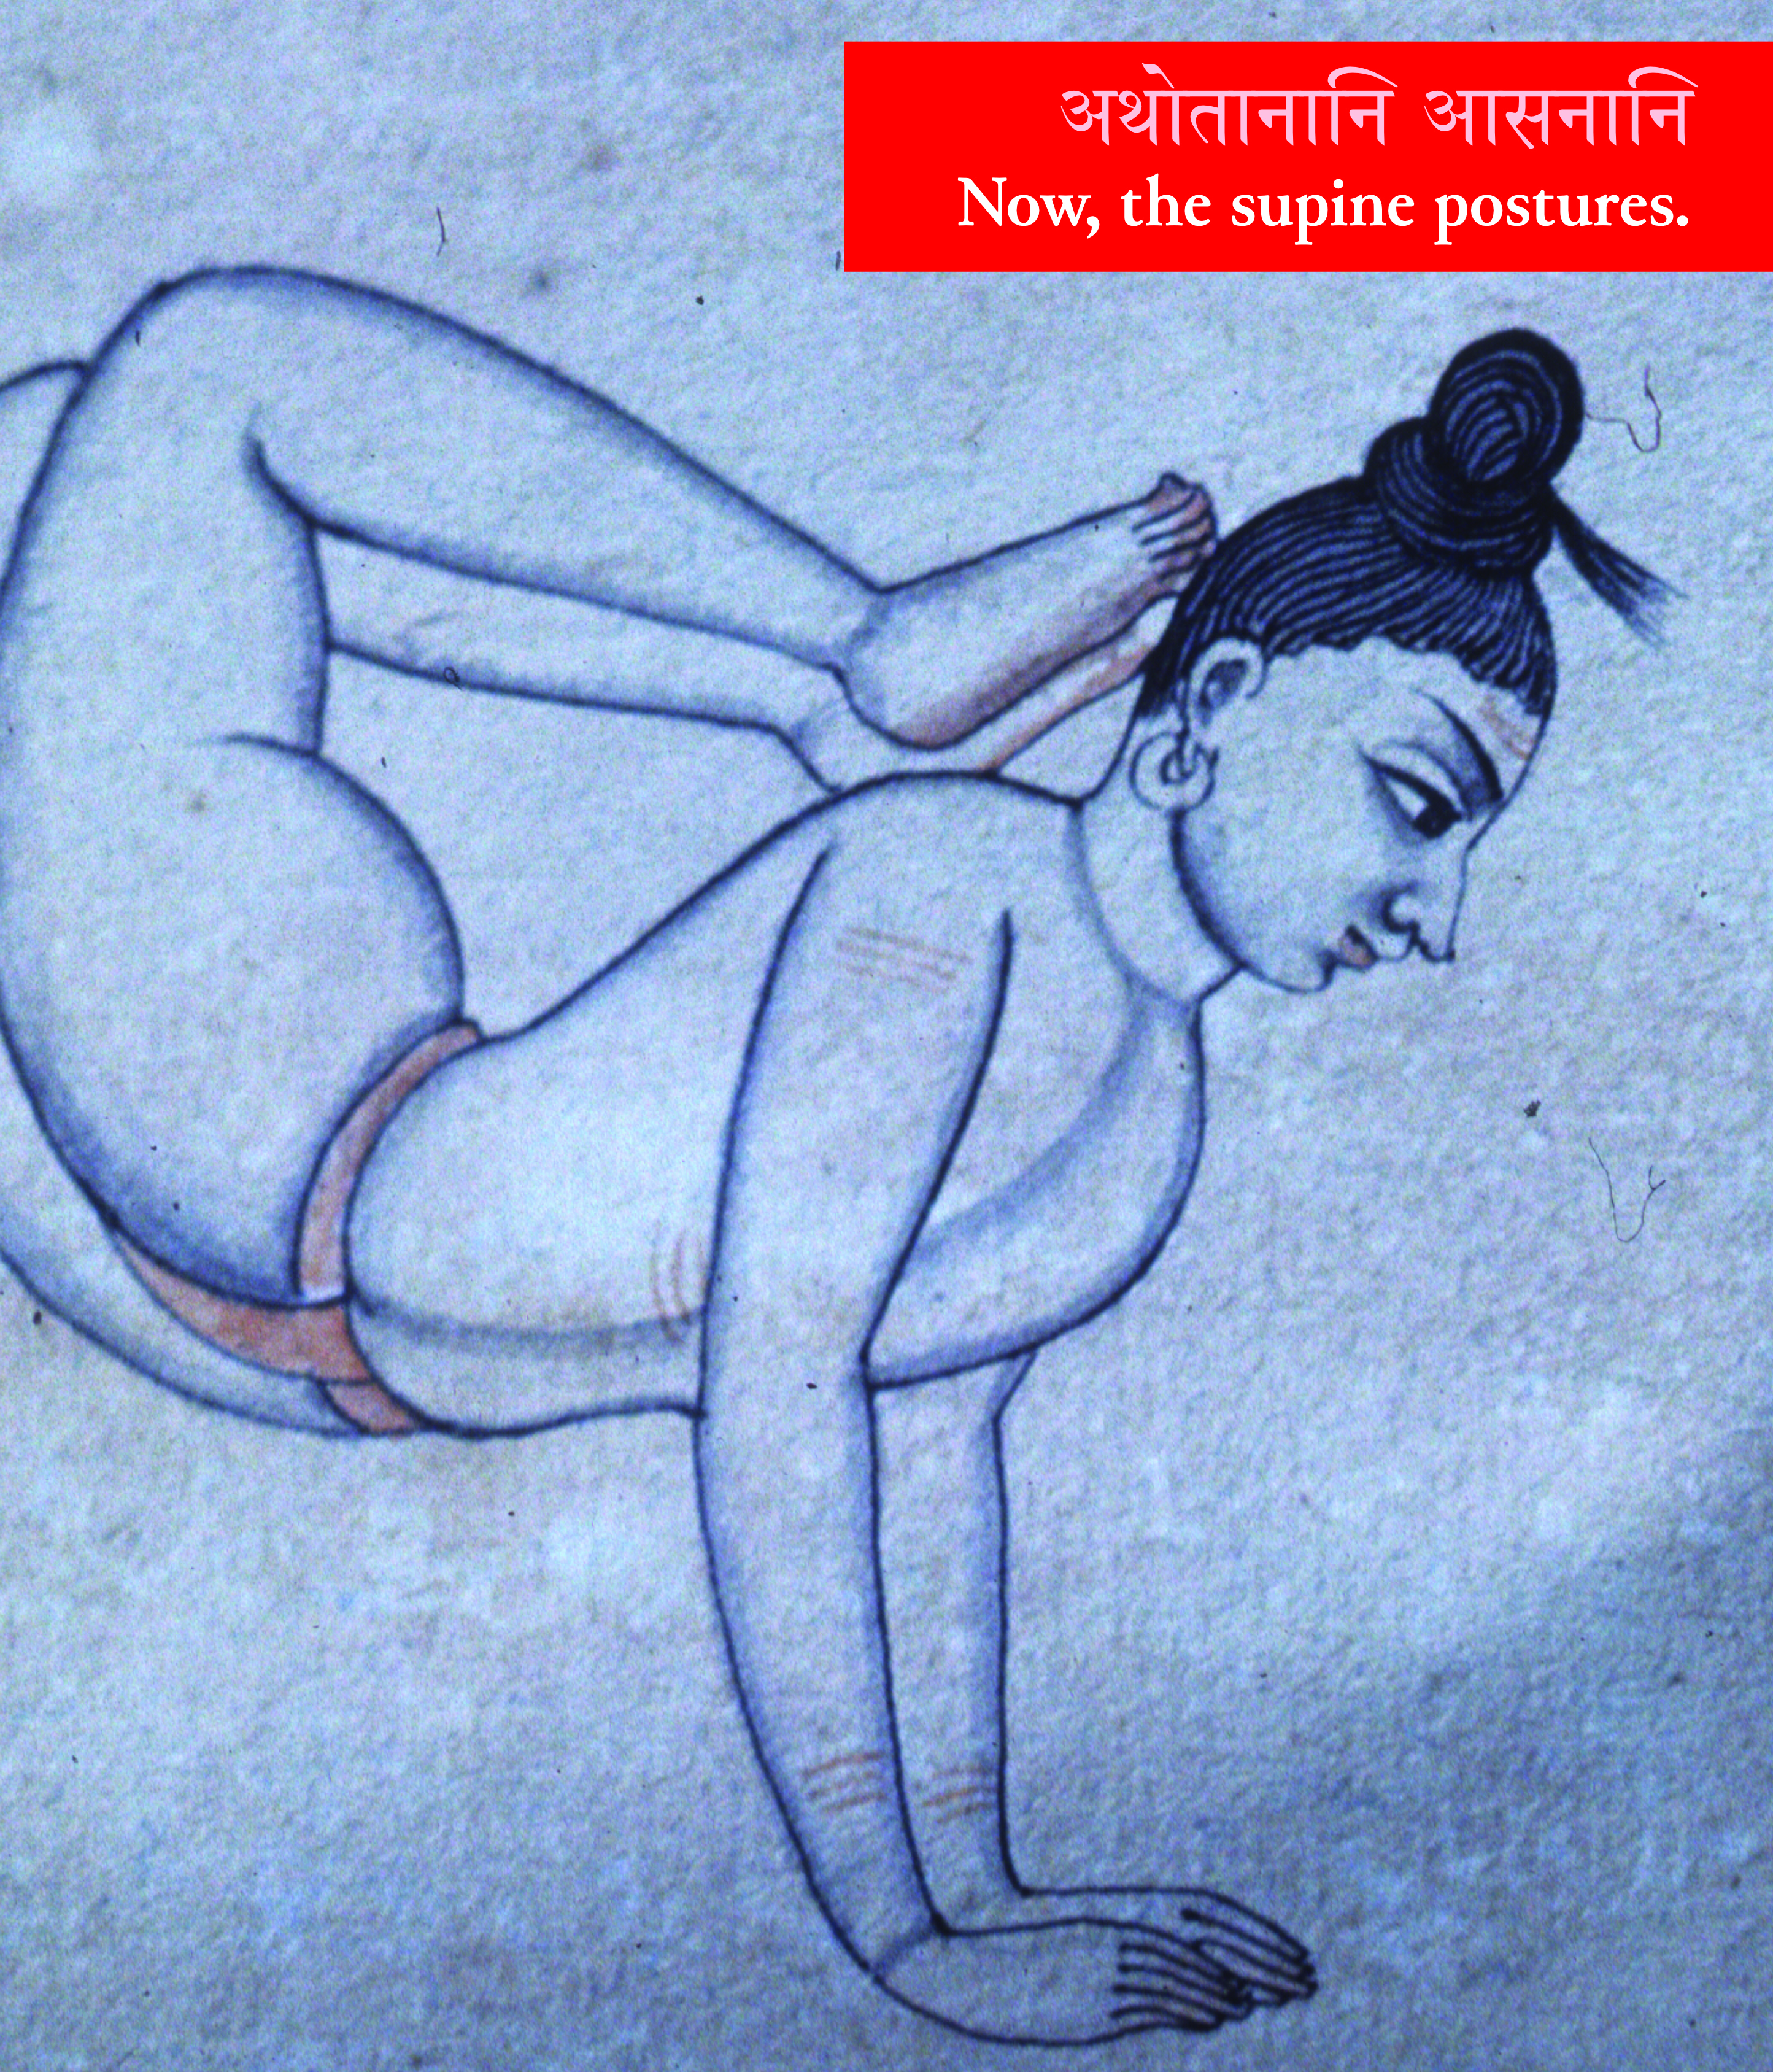
\includegraphics[width=\paperwidth, height=\paperheight, keepaspectratio]{cover2.jpg}
  %};
%\end{tikzpicture}

%~ ~\vfill
%~ \vbox{\vsize=28.575cm
%~ \hbox{\hsize=24.4602cm\noindent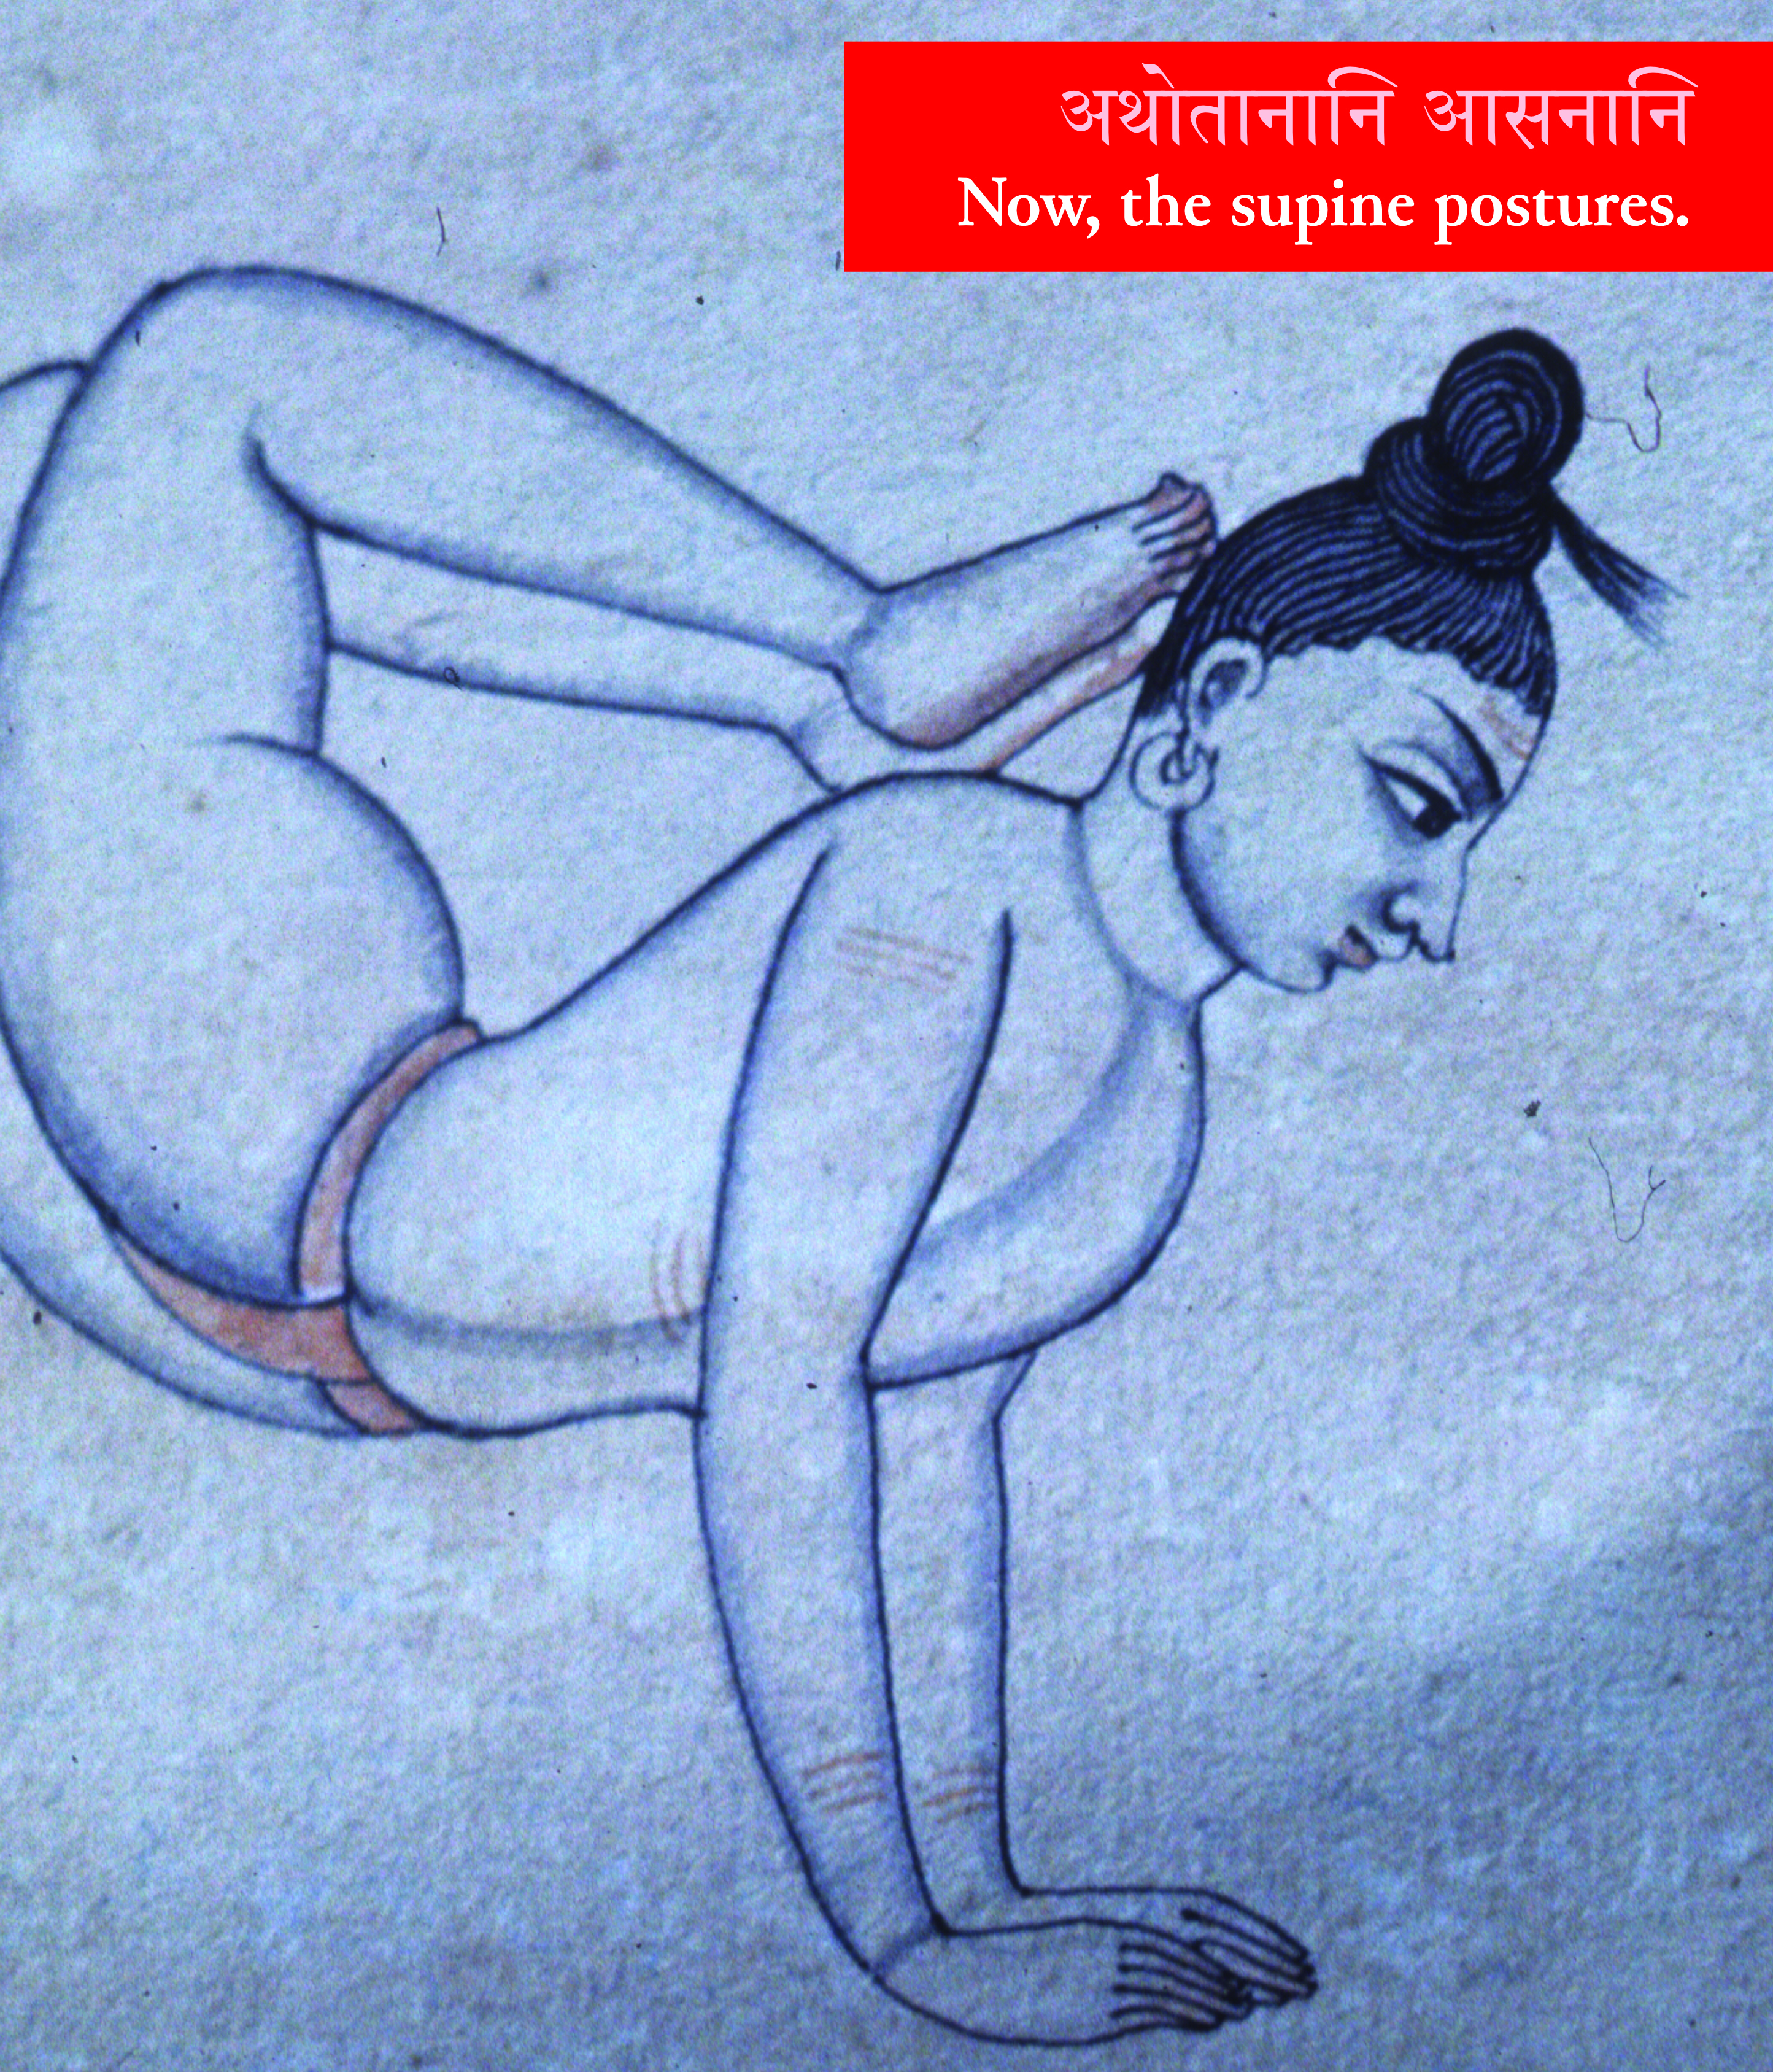
\includegraphics{cover2.jpg}}%
%~ }
%~ \vfill
% new paragraph % beginning of section on āsanas
\newpage

%~ \begin{kan}
%~ \heading{\textkannada{[ಭಂಗಿಗಳು (ಆಸನ)]}} % heading/new section
%~ \bigskip

%~ ಮುಂದೆ, ಆರು ಶುದ್ಧೀಕರಣ ತಂತ್ರಗಳನ್ನು [ಅಭ್ಯಾಸ ಮಾಡುವ] ಸಾಮರ್ಥ್ಯವನ್ನು ಪಡೆಯುವ ಭಂಗಿಗಳನ್ನು ವಿವರಿಸಲಾಗಿದೆ.
%~ \bigskip

%~ \heading{\textkannada{ಈಗ, ಸುಪೈನ್ ಭಂಗಿಗಳು.}} % heading of āsana group 1 
%~ \end{kan}
% [End: Kannada Translation]
% Insert a new section page with beautiful graphic with the words "athottānāni āsanāni (Now, the Supine Postures)", which is the first group of āsanas.
%%%%%%%%%%%%%%%%%%%%%%%
% [Beginning: folio 3r, tiff no. 69]
%\vfill

\newpage
~\vskip 10mm
\centerline{\fcolorbox{plum}{white}{\includegraphics[scale=1]{9_Page_069_1.jpg}}}
\vskip 20mm

% [End: folio 3r, tiff no. 69]
% [Beginning: English Translation]

\begin{sans}
%\begin{multicols}{2}
% [Devanāgarī Transcription]
athottānāni āsanāni\!॥\\
uttānaṃ śayanaṃ kṛtvā aṅgulibhiḥ kandharāṃ baddhvā kūrparau militvā nitambena bhūmiṃ spṛṣṭvā ekaṃ pādaṃ prasārya ekaikena pādena savyadakṣiṇaṃ bhrāmayitvā vṛṣapādakṣepaṃ bhavati\!॥1\!॥
\bigskip

%\rule{\columnwidth}{0pt}
%uttānaṃ śayanaṃ kṛtvā pādau militvā prasārya nitambaṃ bhūmau spṛṣṭvā hastābhyāṃ kandharāṃ\endnote{kandharāṃ] P, kandharaṃ M} baddhvā kumbhakaṃ kṛtvā tiṣṭhet\!। parighāsanaṃ bhavati\!॥2\!॥\\
%\end{multicols}
\end{sans}
\bigskip

\begin{kan}
%\begin{multicols}{2}
% [Beginning: Kannada Translation]
{\color{deepmaroon}{\textkannada{ಉತ್ಥಾನ ಭಂಗಿಗಳು}}} % heading of āsana group 1 

\textkannada{[ಯೋಗಿ] ಬೆನ್ನನ್ನು ಬೆನ್ನಿನೊಂದಿಗೆ ಮಲಗಿಸಿ, ಬೆರಳುಗಳಿಂದ ಕುತ್ತಿಗೆಯನ್ನು ಕಟ್ಟಿಕೊಂಡು, ಮೊಣಕೈಗಳನ್ನು ಜೋಡಿಸಿ, ಪೃಷ್ಠವನ್ನು ನೆಲದ ಮೇಲೆ ಸ್ಪರ್ಶಿಸಿ, ಒಂದು ಕಾಲನ್ನು ಚಾಚಿ ಇನ್ನೊಂದು ಕಾಲನ್ನು ಎಡ ಮತ್ತು ಬಲಕ್ಕೆ ತಿರುಗಿಸಬೇಕು. [ಇದು] ಗೂಳಿಯಂತೆ ಕಾಲನ್ನು ನೇತು ಹಾಕುವುದು [ಭಂಗಿ].}

% new paragraph
%\phantom{\color{deepmaroon}{\textkannada{ಉತ್ಥಾನ ಭಂಗಿಗಳು}}}

%\textkannada{[ಯೋಗಿ] ಬೆನ್ನಿನ ಮೇಲೆ ಮಲಗಿ, ಕಾಲುಗಳನ್ನು ಜೋಡಿಸಿ ಮತ್ತು ಚಾಚಿ, ಪೃಷ್ಠವನ್ನು ನೆಲದ ಮೇಲೆ ಸ್ಪರ್ಶಿಸಿ, ಕುತ್ತಿಗೆಯನ್ನು ಕೈಗಳಿಂದ ಕಟ್ಟಬೇಕು, ಉಸಿರನ್ನು ಹಿಡಿದಿಟ್ಟುಕೊಂಡು ಹಾಗೆಯೇ ಇರಬೇಕು. [ಇದು] ಕಬ್ಬಿಣದ ಸಲಾಕೆಯ ಭಂಗಿ.}
%% [End: Kannada Translation]
%\end{multicols}
\end{kan}
\bigskip

\begin{eng}
%\begin{multicols}{2}
{\color{deepmaroon}{\textenglish{Now, the Supine Postures.}}} % heading of āsana group 1 
\medskip

\vbox{[The yogi] should lie supine,  bind the neck with the fingers, join the elbows, touch the buttocks on the ground, extend one leg and rotate the other leg to the left and right. [This] is the Pawing the Leg like a Bull [Pose].}
\bigskip

%\phantom{\heading{\textenglish{Now, the Supine Postures.}}}
%[The yogi] should lie supine, join and extend the legs, touch the buttocks on the ground, bind the neck with the hands, hold the breath and remain thus. [This] is the Iron-bar Pose.
%\end{multicols}
\end{eng}


% [End: English Translation]

\newpage
~\vskip 10mm
\centerline{\fcolorbox{plum}{white}{\includegraphics[scale=1]{9_Page_069_2.jpg}}}
\vskip 20mm

% [End: folio 3r, tiff no. 69]
% [Beginning: English Translation]

\begin{sans}
%\begin{multicols}{2}
% [Devanāgarī Transcription]
%athottānāni āsanāni\!॥\\
%uttānaṃ śayanaṃ kṛtvā aṅgulibhiḥ kandharāṃ baddhvā kūrparau militvā nitambena bhūmiṃ spṛṣṭvā ekaṃ pādaṃ prasārya ekaikena pādena savyadakṣiṇaṃ bhrāmayitvā vṛṣapādakṣepaṃ bhavati\!॥1\!॥
%\bigskip

%\rule{\columnwidth}{0pt}
uttānaṃ śayanaṃ kṛtvā pādau militvā prasārya nitambaṃ bhūmau spṛṣṭvā hastābhyāṃ kandharāṃ\endnote{kandharāṃ] P, kandharaṃ M} baddhvā kumbhakaṃ kṛtvā tiṣṭhet\!। parighāsanaṃ bhavati\!॥2\!॥\\
%\end{multicols}
\end{sans}
\bigskip

\begin{kan}
%\begin{multicols}{2}
% [Beginning: Kannada Translation]
%{\color{deepmaroon}{\textkannada{ಉತ್ಥಾನ ಭಂಗಿಗಳು}}} % heading of āsana group 1 

%\textkannada{[ಯೋಗಿ] ಬೆನ್ನನ್ನು ಬೆನ್ನಿನೊಂದಿಗೆ ಮಲಗಿಸಿ, ಬೆರಳುಗಳಿಂದ ಕುತ್ತಿಗೆಯನ್ನು ಕಟ್ಟಿಕೊಂಡು, ಮೊಣಕೈಗಳನ್ನು ಜೋಡಿಸಿ, ಪೃಷ್ಠವನ್ನು ನೆಲದ ಮೇಲೆ ಸ್ಪರ್ಶಿಸಿ, ಒಂದು ಕಾಲನ್ನು ಚಾಚಿ ಇನ್ನೊಂದು ಕಾಲನ್ನು ಎಡ ಮತ್ತು ಬಲಕ್ಕೆ ತಿರುಗಿಸಬೇಕು. [ಇದು] ಗೂಳಿಯಂತೆ ಕಾಲನ್ನು ನೇತು ಹಾಕುವುದು [ಭಂಗಿ].}

% new paragraph
%\phantom{\color{deepmaroon}{\textkannada{ಉತ್ಥಾನ ಭಂಗಿಗಳು}}}

\textkannada{[ಯೋಗಿ] ಬೆನ್ನಿನ ಮೇಲೆ ಮಲಗಿ, ಕಾಲುಗಳನ್ನು ಜೋಡಿಸಿ ಮತ್ತು ಚಾಚಿ, ಪೃಷ್ಠವನ್ನು ನೆಲದ ಮೇಲೆ ಸ್ಪರ್ಶಿಸಿ, ಕುತ್ತಿಗೆಯನ್ನು ಕೈಗಳಿಂದ ಕಟ್ಟಬೇಕು, ಉಸಿರನ್ನು ಹಿಡಿದಿಟ್ಟುಕೊಂಡು ಹಾಗೆಯೇ ಇರಬೇಕು. [ಇದು] ಕಬ್ಬಿಣದ ಸಲಾಕೆಯ ಭಂಗಿ.}
%% [End: Kannada Translation]
%\end{multicols}
\end{kan}
\bigskip

\begin{eng}
%\begin{multicols}{2}
%{\color{deepmaroon}{\textenglish{Now, the Supine Postures.}}} % heading of āsana group 1 
%\medskip

%\vbox{[The yogi] should lie supine,  bind the neck with the fingers, join the elbows, touch the buttocks on the ground, extend one leg and rotate the other leg to the left and right. [This] is the Pawing the Leg like a Bull [Pose].}
%\bigskip

%\phantom{\heading{\textenglish{Now, the Supine Postures.}}}
[The yogi] should lie supine, join and extend the legs, touch the buttocks on the ground, bind the neck with the hands, hold the breath and remain thus. [This] is the Iron-bar Pose.
%\end{multicols}
\end{eng}


% [End: English Translation]
\vfill
\newpage


~\vskip 10mm
\centerline{\fcolorbox{plum}{white}{\includegraphics[scale=0.59]{9_Page_070.jpg}}}
\vskip 20mm

%%%%%%%%%%%%%%%%%%%%%%
% [Beginning: folio 3v, tiff no. 70]
% [Devanāgarī Transcription]

\begin{sans}
\begin{multicols}{2}
\vbox{uttānaṃ śayanaṃ kūrparadvayaṃ nābhau sthāpayitvā ekaikaṃ hastaṃ prasārya nāsikāyāmaṅguṣṭhapradeśena dhṛtvā tallakṣyeṇa jaghana\-pradeśena dhṛtvā sthāpayet\!। paraśvāsanaṃ\endnote{paraśvāsanaṃ] M(ac) P, paraśvadhāsanaṃ M(pc)} bhavati\!॥3\!॥}
\bigskip

uttānaṃ śayanamekaikaṃ pādaṃ grīvāyāṃ vinyasya itarahastena pādāgraṃ gṛhītvā itarapādahastau lambīkṛtya tiṣṭhet\!। anantāsanaṃ bhavati\!॥4\!॥
% [End: folio 3v, tiff no. 70]
\end{multicols}
\end{sans}
\bigskip

\begin{kan}
\begin{multicols}{2}
% [Beginning: Kannada Translation]
\textkannada{[ಯೋಗಿ] ಬೆನ್ನಿನ ಮೇಲೆ ಮಲಗಬೇಕು, ಮೊಣಕೈಗಳನ್ನು ಹೊಕ್ಕುಳಿನ ಮೇಲೆ ಇಡಬೇಕು, ಒಂದೊಂದಾಗಿ ಕೈಗಳನ್ನು ಚಾಚಬೇಕು, ಮೂಗನ್ನು [ಇನ್ನೊಂದು ಕೈಯ] ಹೆಬ್ಬೆರಳಿನಿಂದ ಹಿಡಿದು ಅದರ ಮೇಲೆ ದೃಷ್ಟಿ ಹಾಯಿಸಬೇಕು, ಅದೇ ಸಮಯದಲ್ಲಿ ಸೊಂಟದ ಭಾಗದಿಂದ [ಸ್ಥಾನವನ್ನು] ಬೆಂಬಲಿಸಬೇಕು ಮತ್ತು ಹಾಗೆಯೇ ಇರಬೇಕು. [ಇದು] ಹ್ಯಾಚೆಟ್ ಭಂಗಿ.}
\bigskip

\textkannada{[ಯೋಗಿ] ಬೆನ್ನಿನ ಮೇಲೆ ಮಲಗಿ, ಒಂದು ಪಾದವನ್ನು ಕುತ್ತಿಗೆಯ ಹಿಂಭಾಗದಲ್ಲಿ ಇರಿಸಿ, ಇನ್ನೊಂದು ಕೈಯಿಂದ ಆ ಪಾದದ ಬೆರಳುಗಳನ್ನು ಹಿಡಿದು, ಇನ್ನೊಂದು ಪಾದ ಮತ್ತು ಕೈಯನ್ನು ಚಾಚಬೇಕು. ಅವನು ಹೀಗೆಯೇ ಇರಬೇಕು [ತದನಂತರ ಇನ್ನೊಂದು ಪಾದವನ್ನು ಕುತ್ತಿಗೆಯ ಮೇಲೆ ಇರಿಸಿ ಅದನ್ನು ಪುನರಾವರ್ತಿಸಬೇಕು]. [ಇದು] ಅನಂತನ ಭಂಗಿ.}
\end{multicols}
\end{kan}
\bigskip

\begin{eng}
\begin{multicols}{2}
\phantom{i}[The yogi] should lie supine, place the elbows on the navel, extend one hand at a time, hold the nose by the thumb [of the other hand] with the gaze on it, while supporting [the position] with the region of the hips, and remain thus. [This] is the Hatchet Pose.
\bigskip

[The yogi] should lie supine, fix one foot on [the back of] the neck, grasp the toes of [that] foot with the other hand, and stretch out the other foot and hand. He should remain thus [and then repeat it with the other foot on the neck]. [This] is Ananta’s Pose.
% [End: English Translation]
\end{multicols}
\end{eng}
\bigskip

\vfill
\newpage

